\documentclass{beamer}
\usetheme{default}
\usepackage[italian]{babel}
%\usepackage{t1enc}
\usepackage{pgfpages}
\usepackage{listings}
%\pgfpagelayout{2 on 1}[a4paper]

%\usepackage{../../common/espacs}
\lstset
{
  language=[ISO]C++,                       % The default language
  basicstyle=\sf,                          % The basic style
  keywordstyle=\color{blue}\bfseries,      % Set keyword style
  commentstyle=\color{darkgreen}\itshape,  % Set comment style
  extendedchars=true                       % Allow extended characters
}

\setbeamercovered{transparent}

\begin{document}

%---------------------------------------------------------------------------------

\begin{frame}[fragile]

    Breve introduzione ad Eclipse.

\end{frame}

%---------------------------------------------------------------------------------

\begin{frame}[fragile]

    \frametitle{Eclipse}

    Per ottenere Eclipse andare sul sito internet

    \begin{verbatim}
        http://www.eclipse.org/downloads/
    \end{verbatim}

    E scaricare il pacchetto

    \begin{figure}
        \centering
        
\includegraphics[width=0.5\textwidth]{./images/eclipselogo}
    \end{figure}

    Scompattare il pacchetto e lanciare Eclipse.

\end{frame}

%---------------------------------------------------------------------------------

\begin{frame}[fragile]

    \frametitle{Eclipse: creare un nuovo progetto}

    \begin{figure}
        \centering
        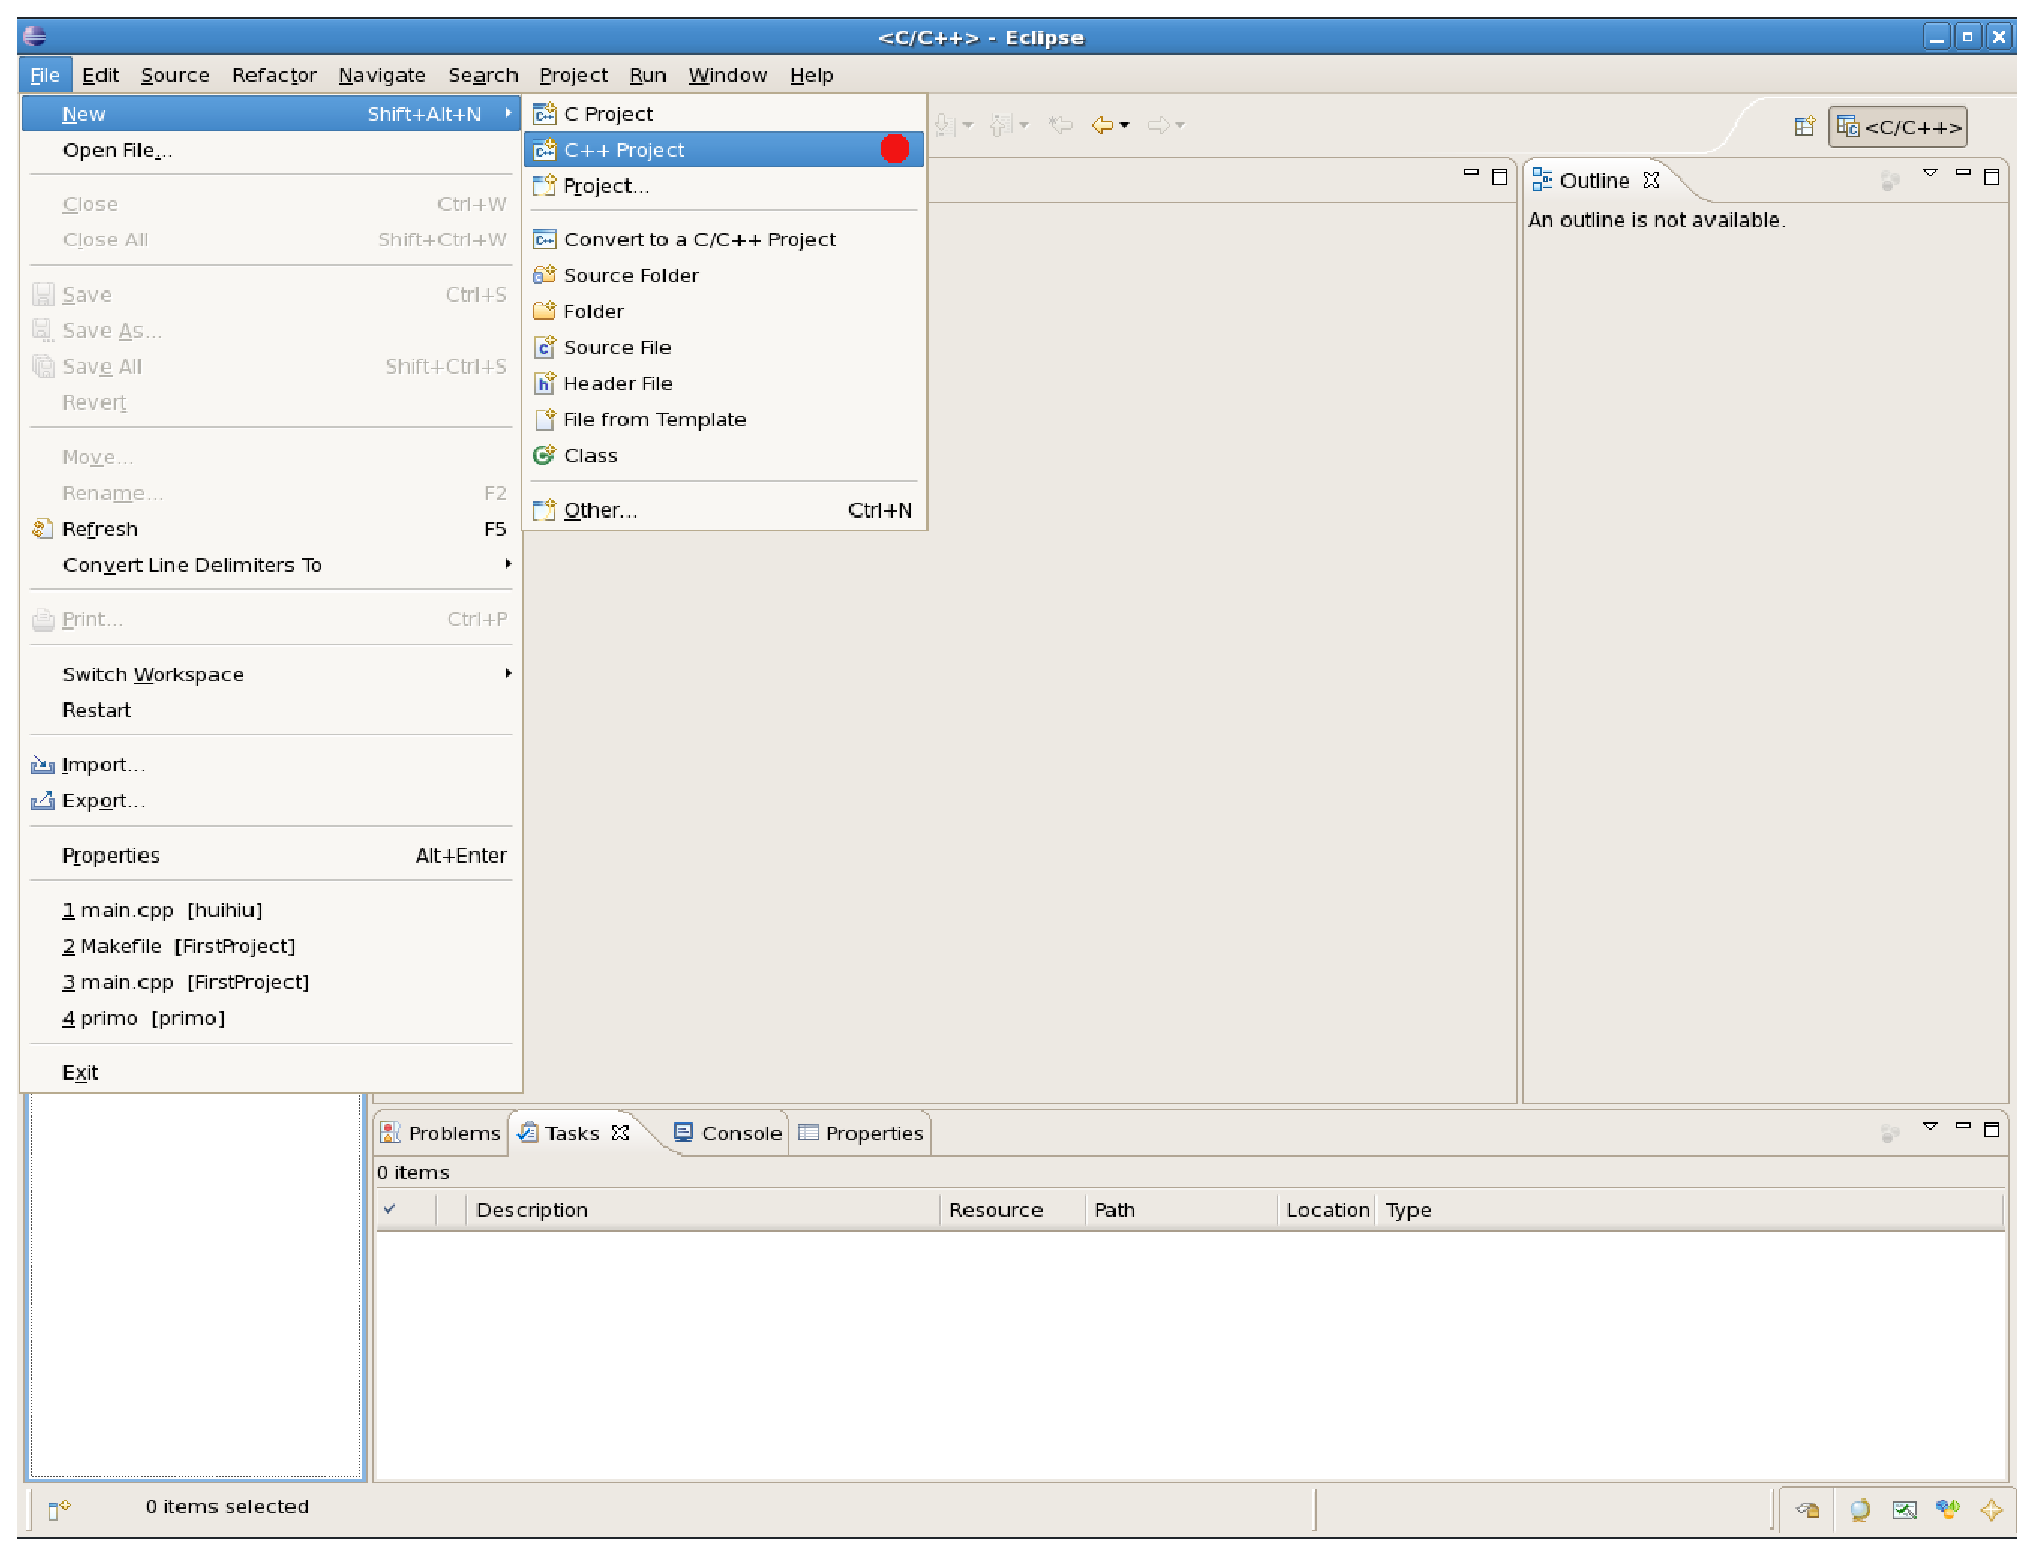
\includegraphics[width=0.95\textwidth]{./images/eclipse1}
    \end{figure}

\end{frame}

%---------------------------------------------------------------------------------

\begin{frame}[fragile]

    \frametitle{Eclipse: inserire nome, compilatore e senza Makefile automatico}

    \begin{figure}
        \centering
        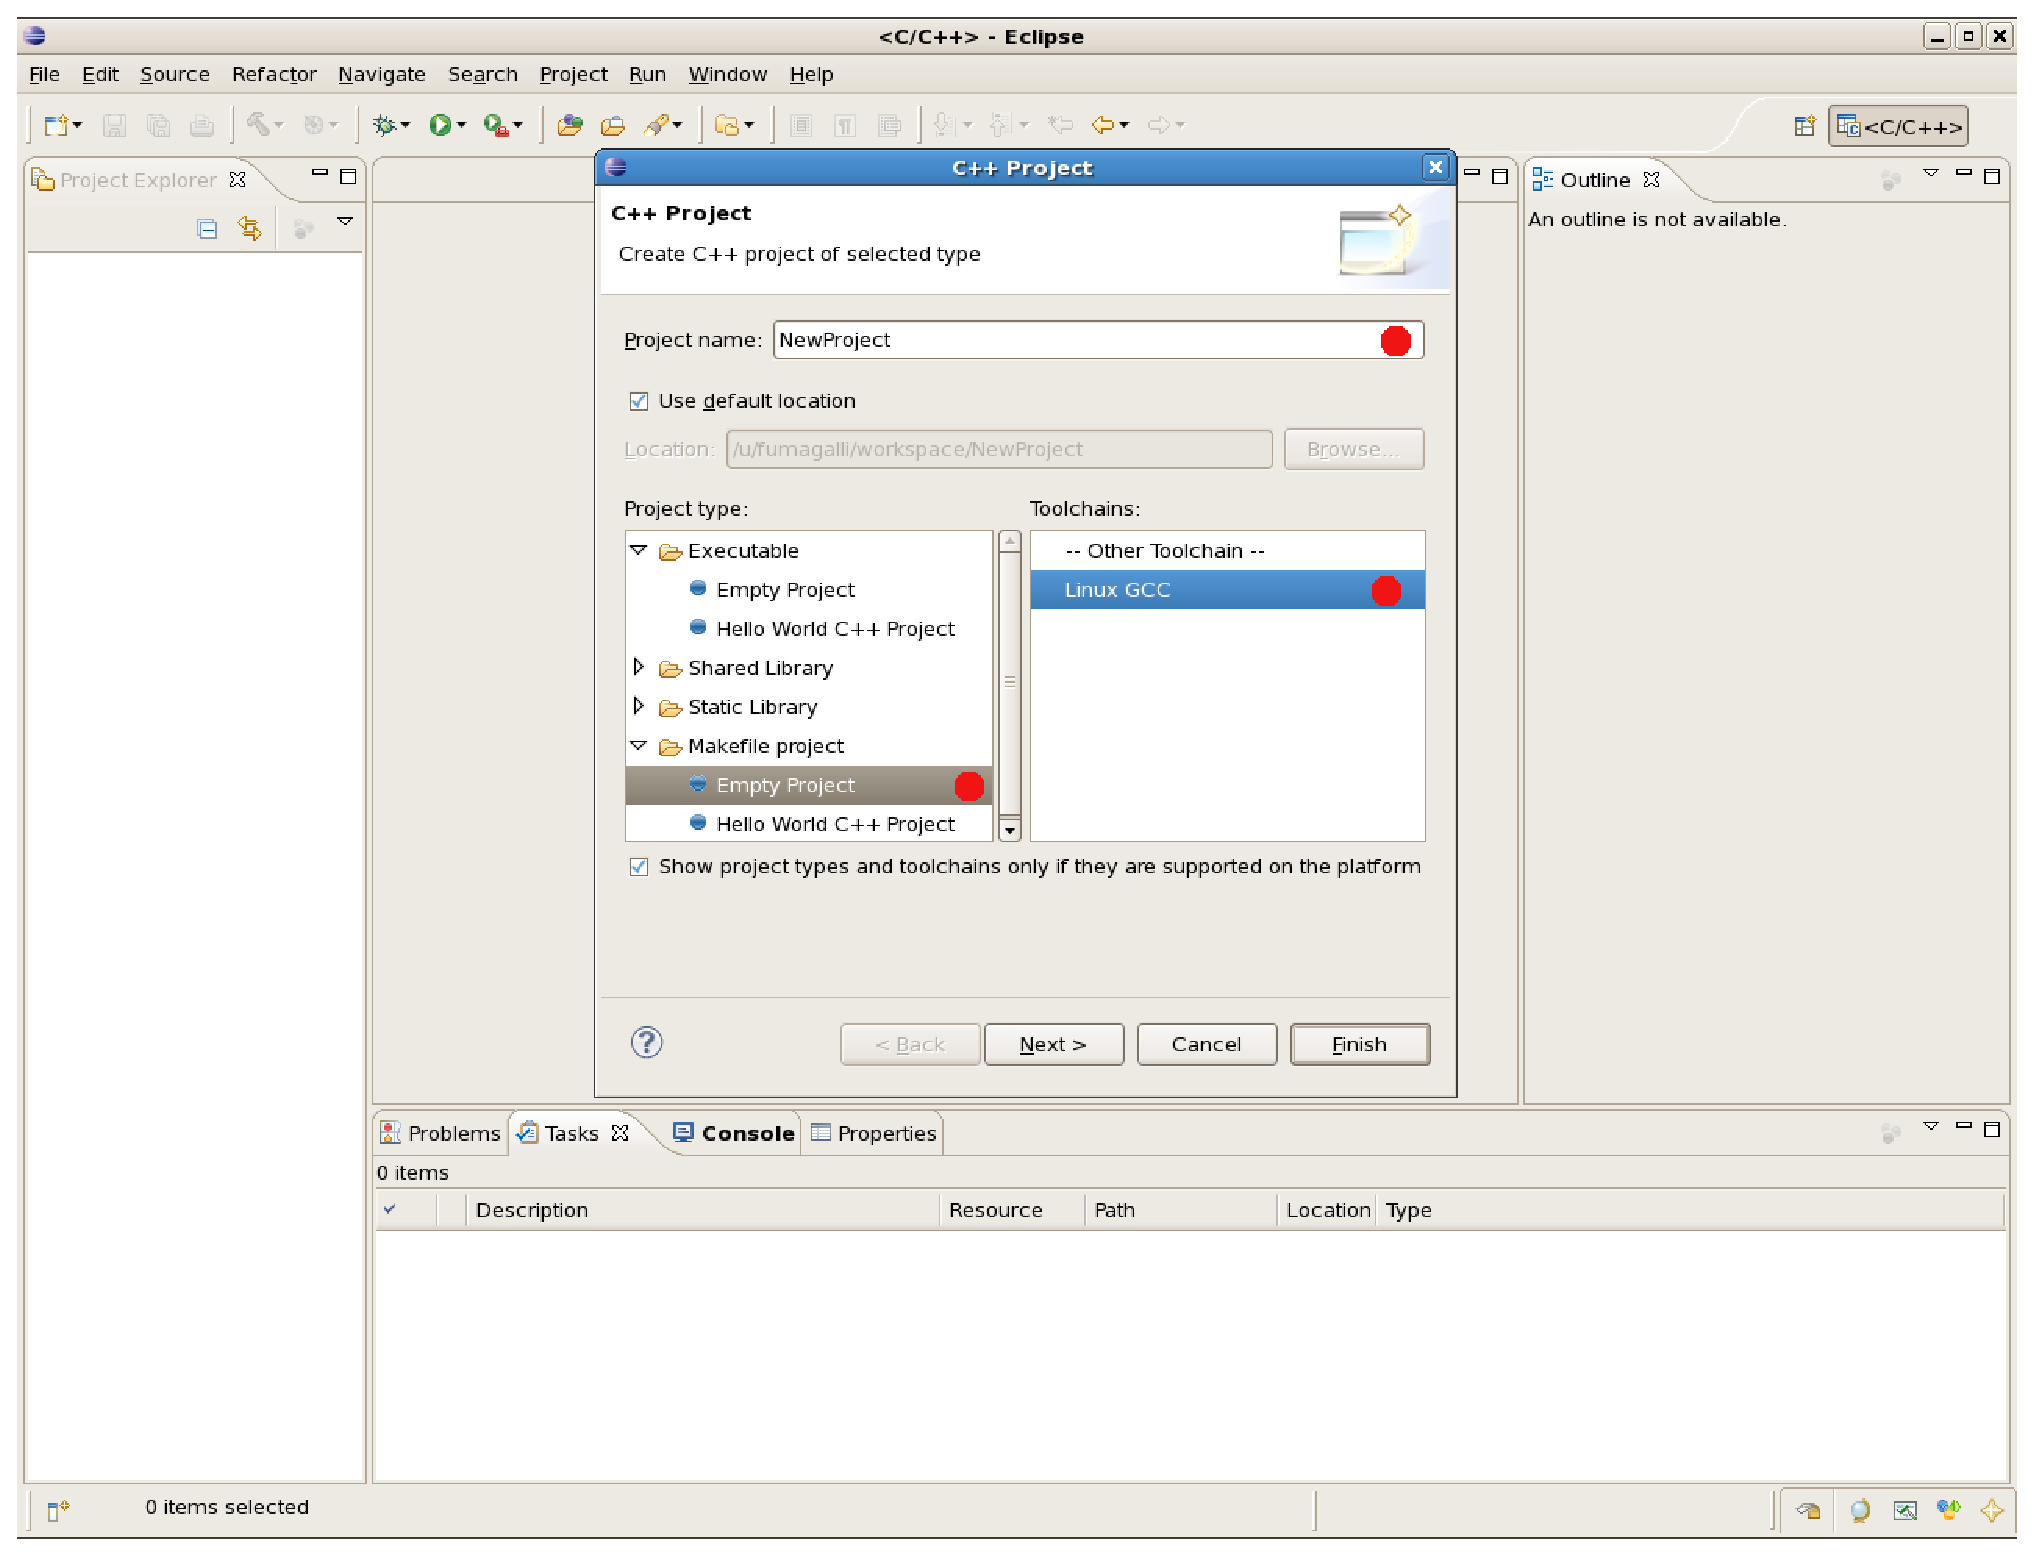
\includegraphics[width=0.95\textwidth]{./images/eclipse2}
    \end{figure}

\end{frame}

%---------------------------------------------------------------------------------

\begin{frame}[fragile]

    \frametitle{Eclipse: inserire un file .cpp}

    \begin{figure}
        \centering
        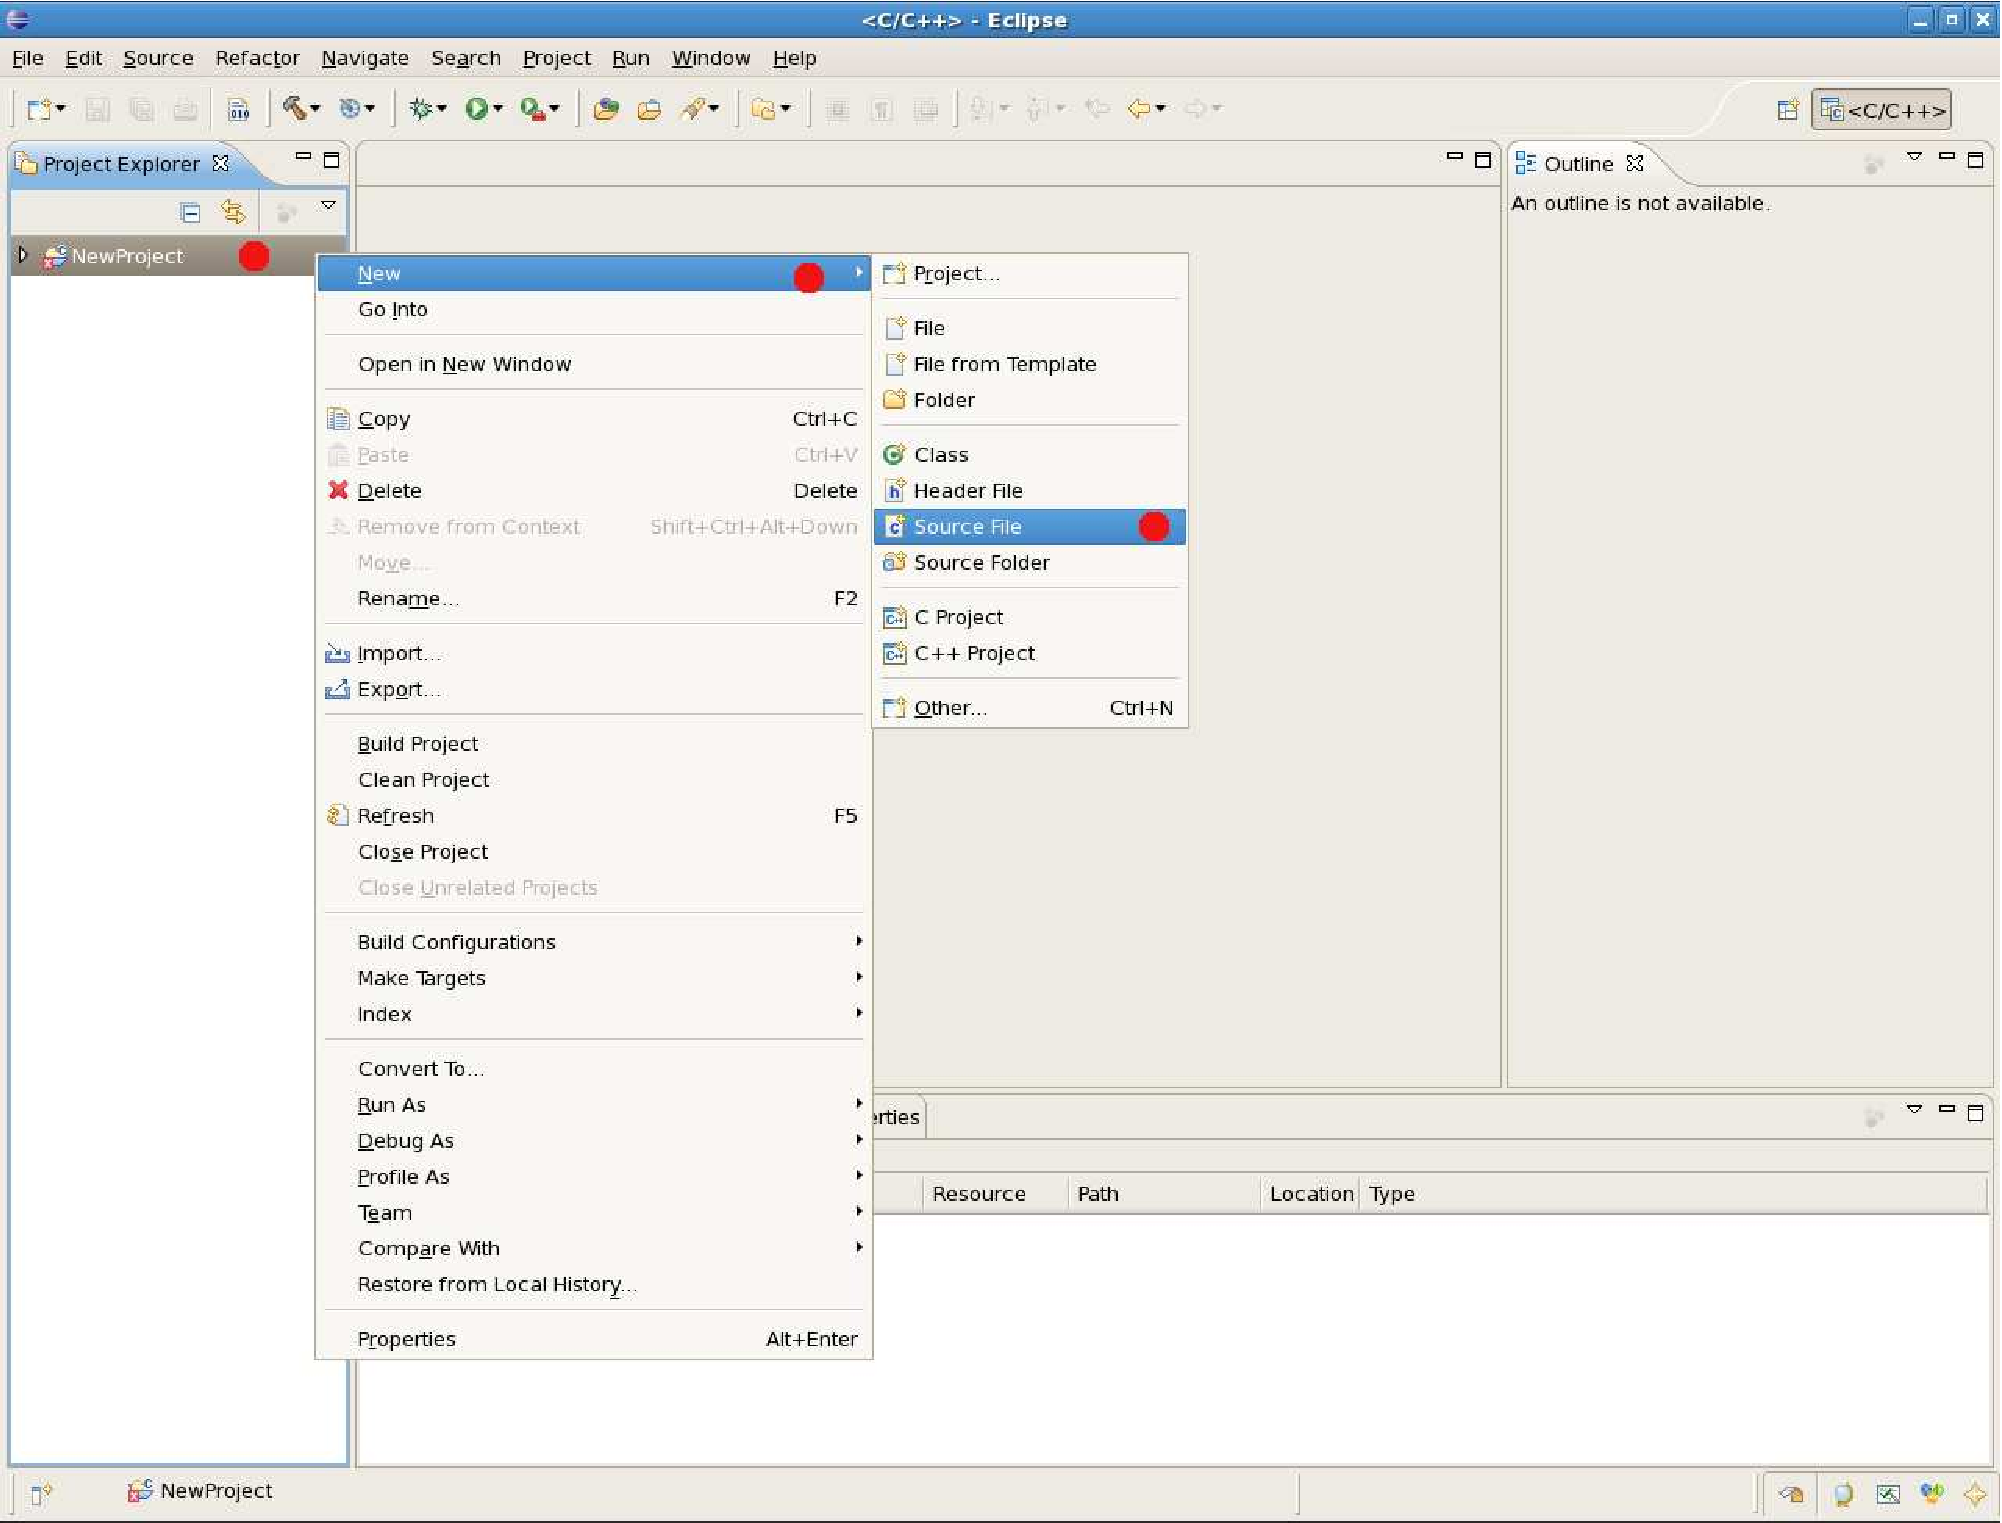
\includegraphics[width=0.95\textwidth]{./images/eclipse3}
    \end{figure}

\end{frame}

%---------------------------------------------------------------------------------

\begin{frame}[fragile]

    \frametitle{Eclipse: inserire il nome del file sorgente}

    \begin{figure}
        \centering
        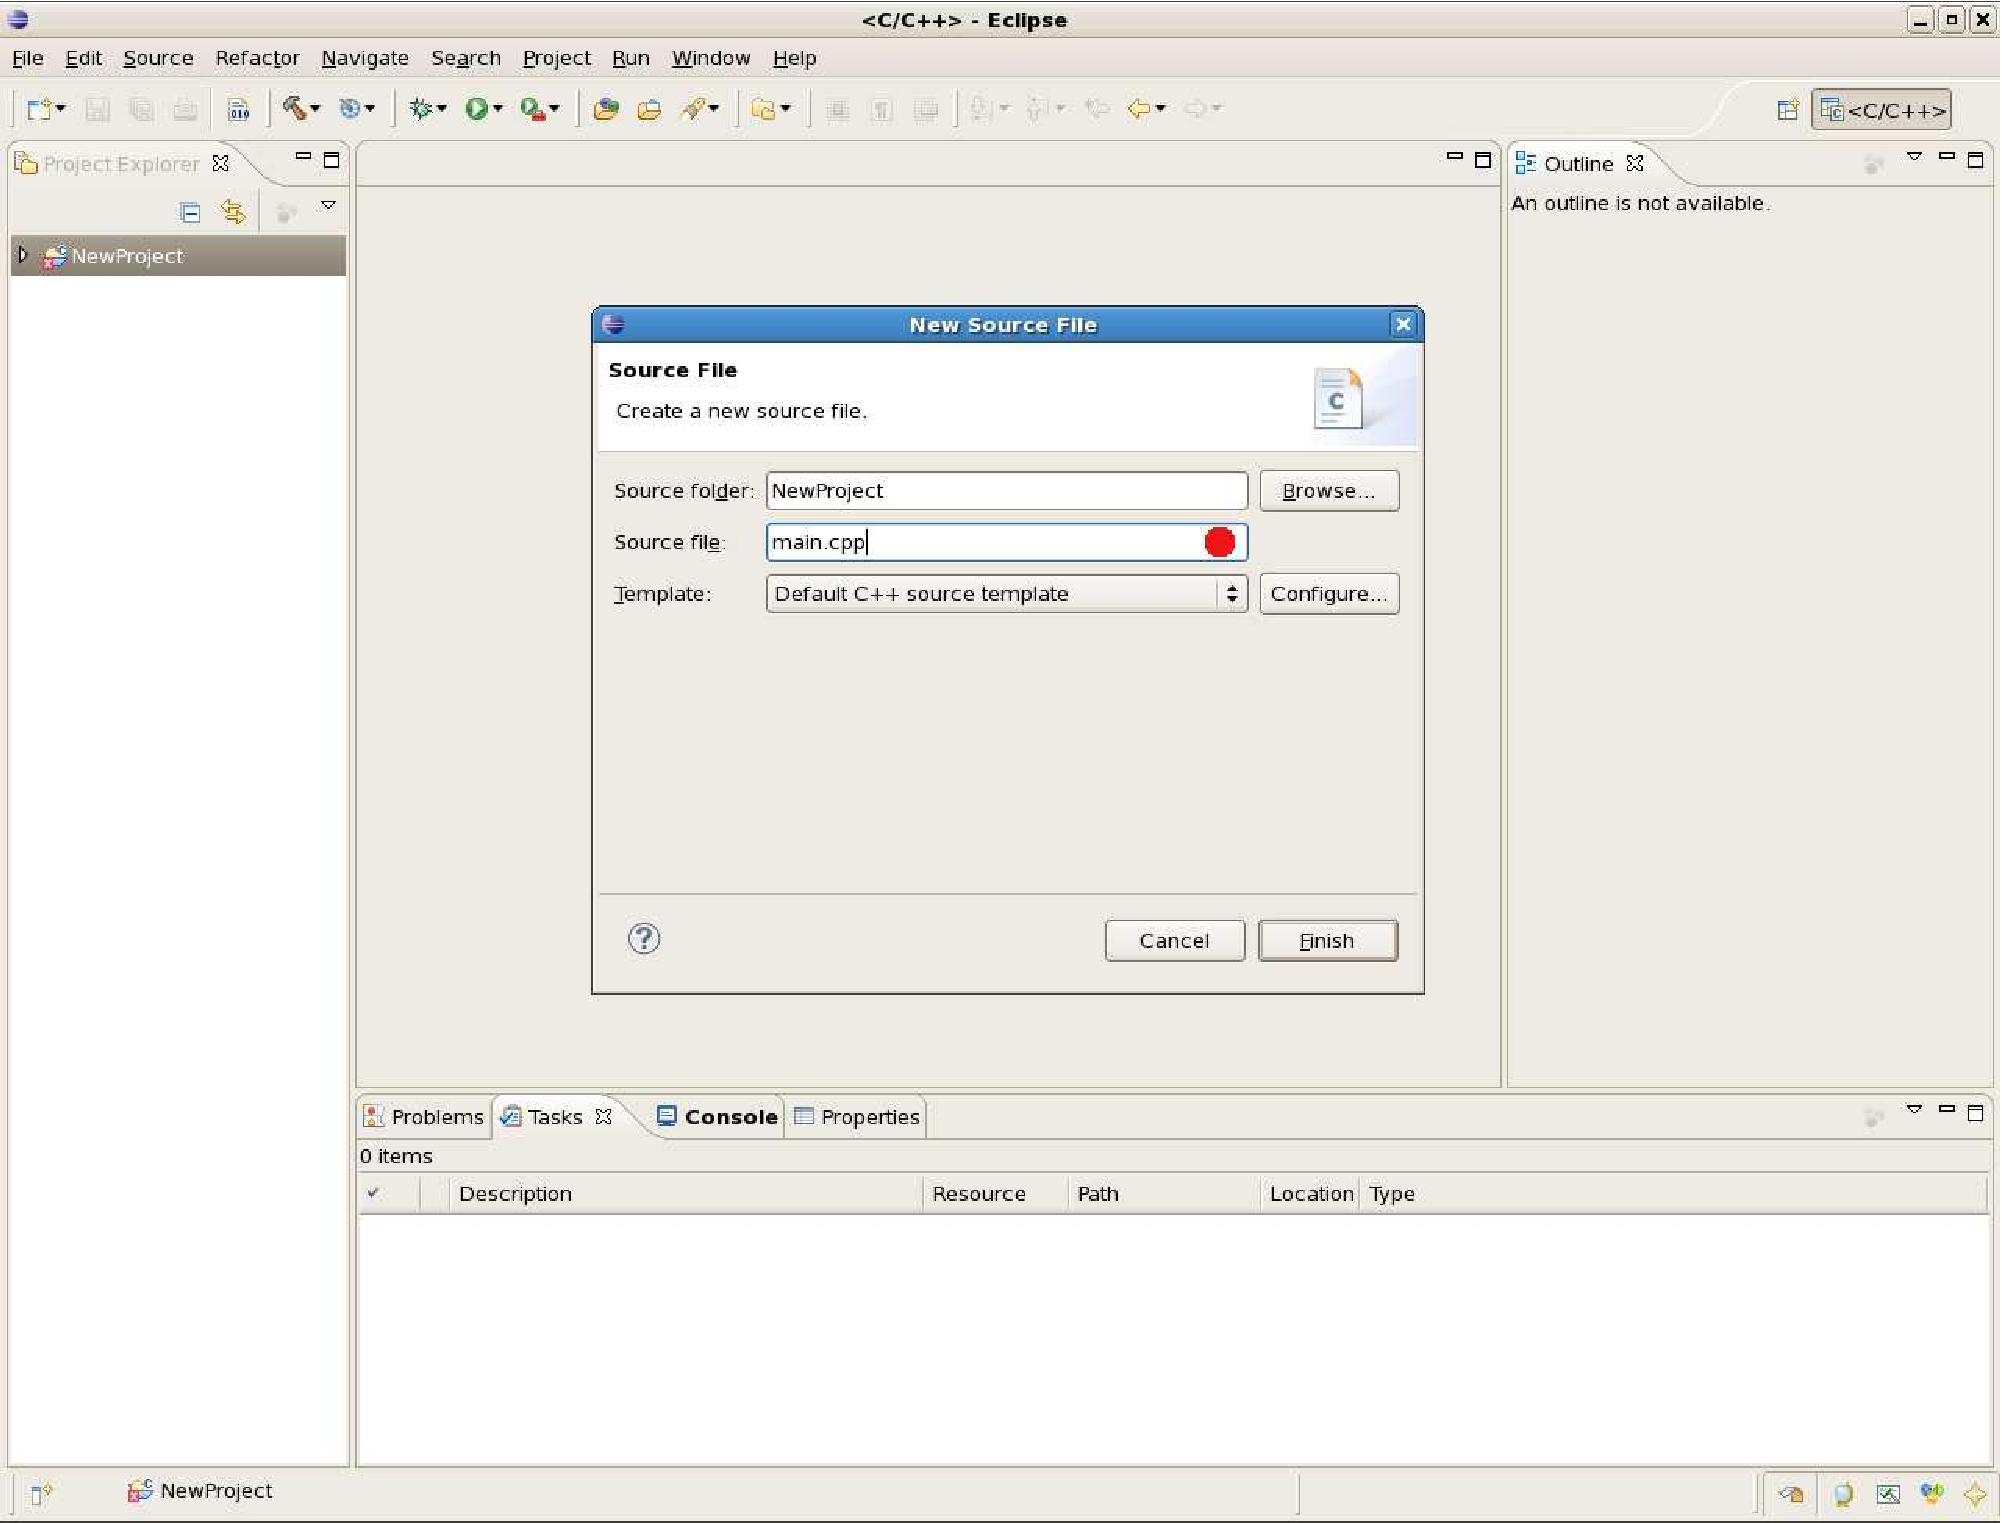
\includegraphics[width=0.95\textwidth]{./images/eclipse4}
    \end{figure}

\end{frame}

%---------------------------------------------------------------------------------

\begin{frame}[fragile]

    \frametitle{Eclipse: esempio programma}

    \begin{figure}
        \centering
        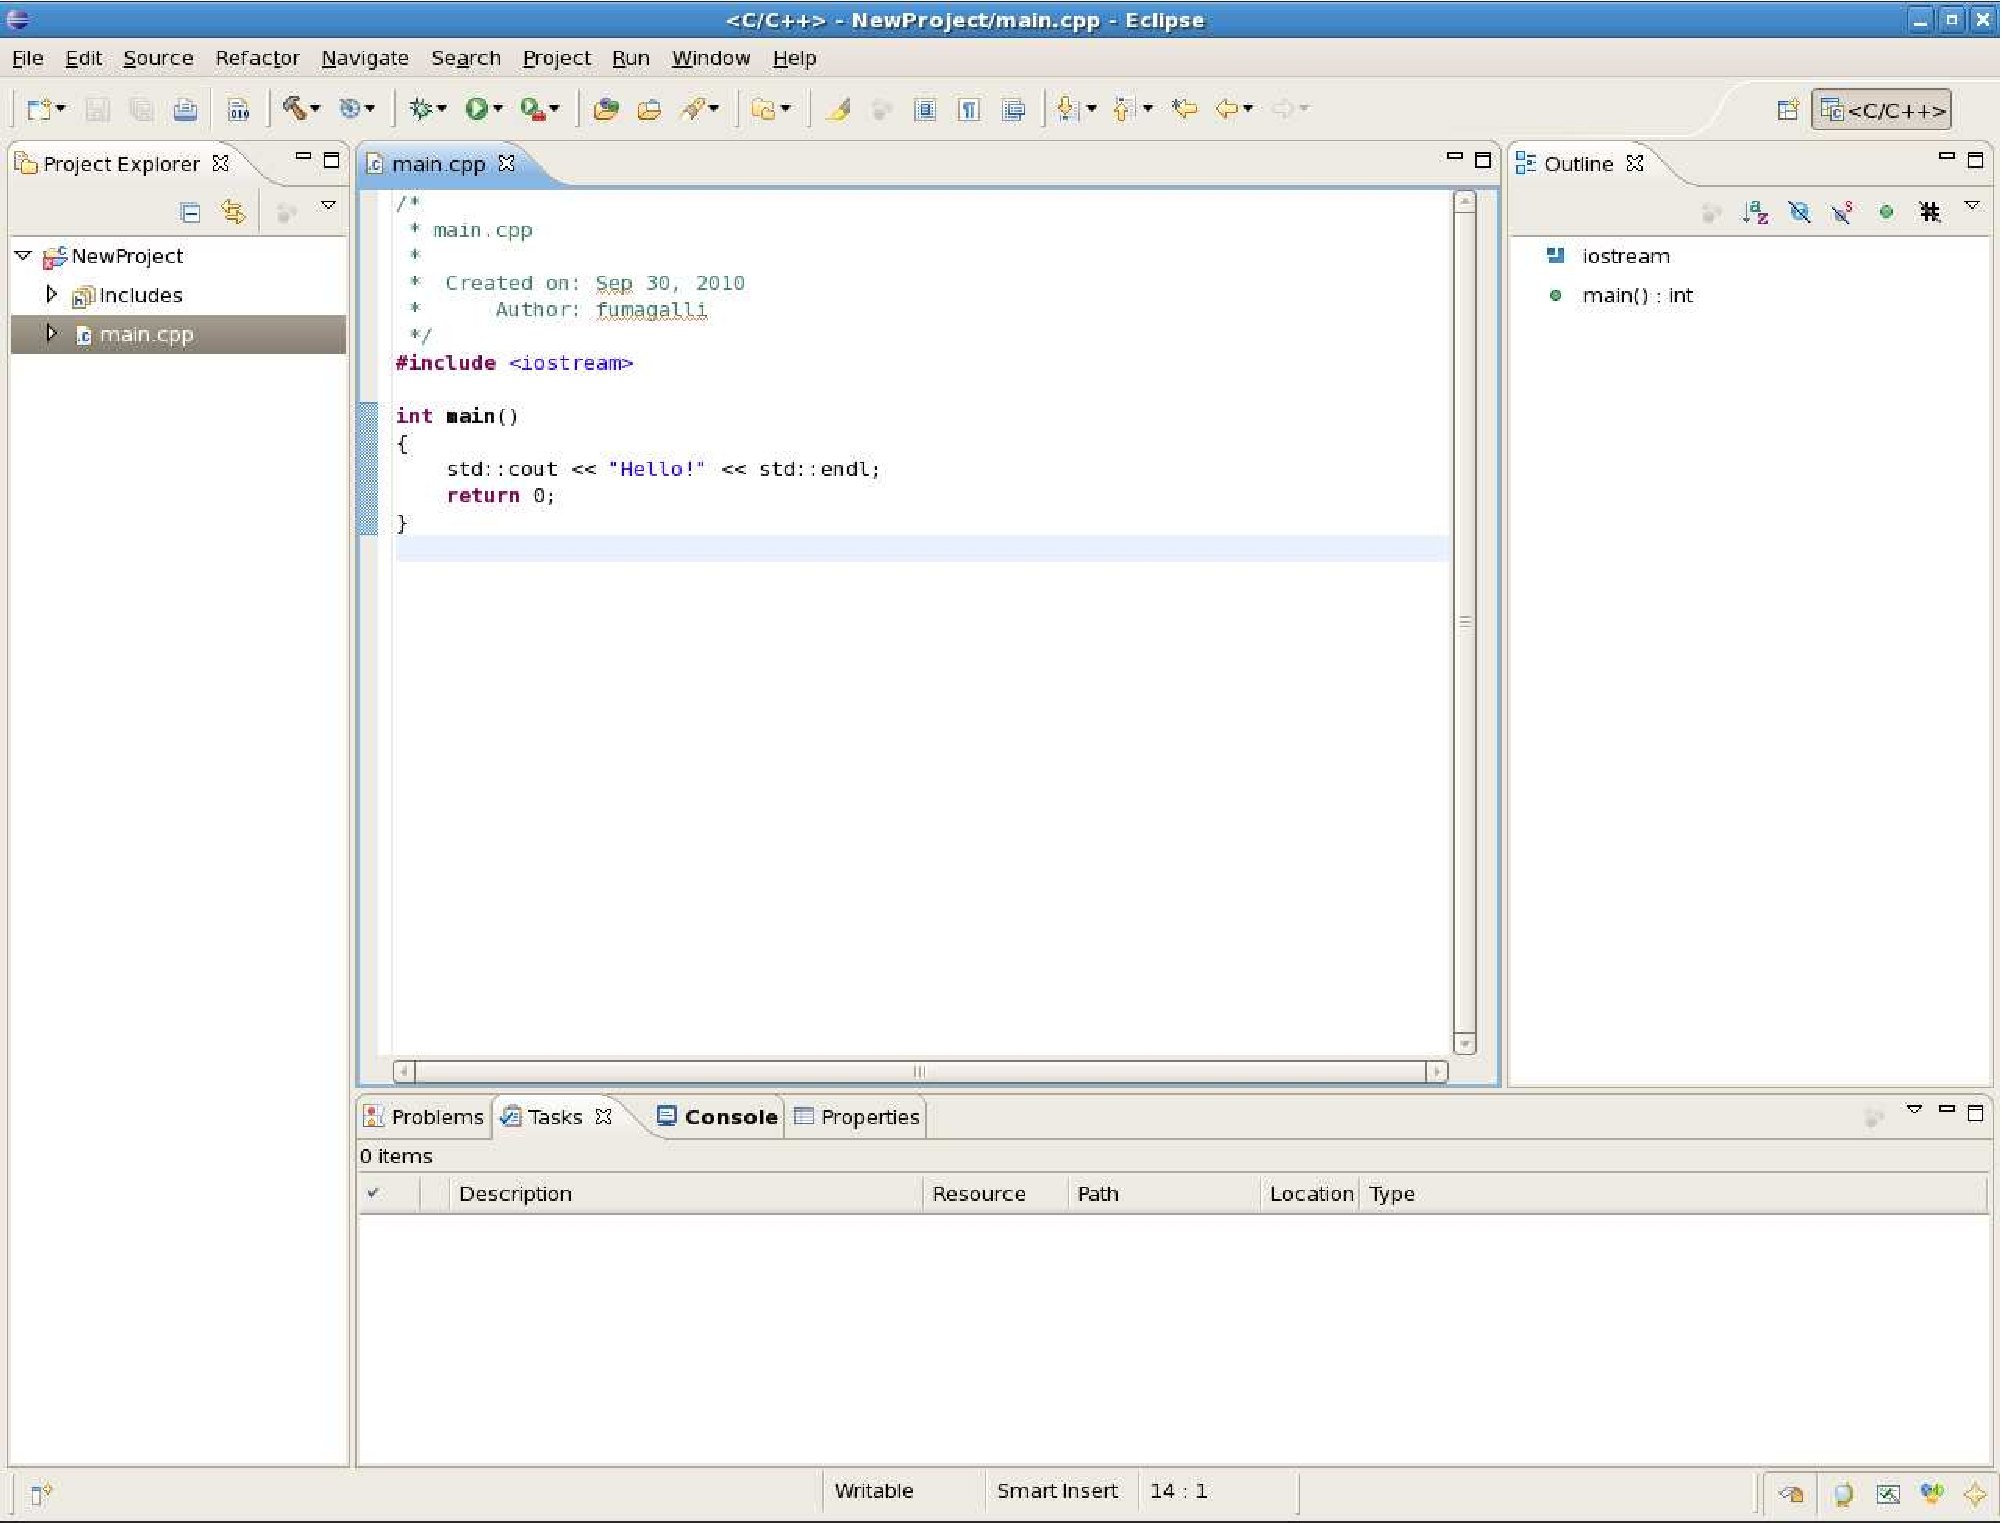
\includegraphics[width=0.95\textwidth]{./images/eclipse5}
    \end{figure}

\end{frame}

%---------------------------------------------------------------------------------

\begin{frame}[fragile]

    \frametitle{Eclipse: per compilare bisogna creare un Makefile}

    \begin{figure}
        \centering
        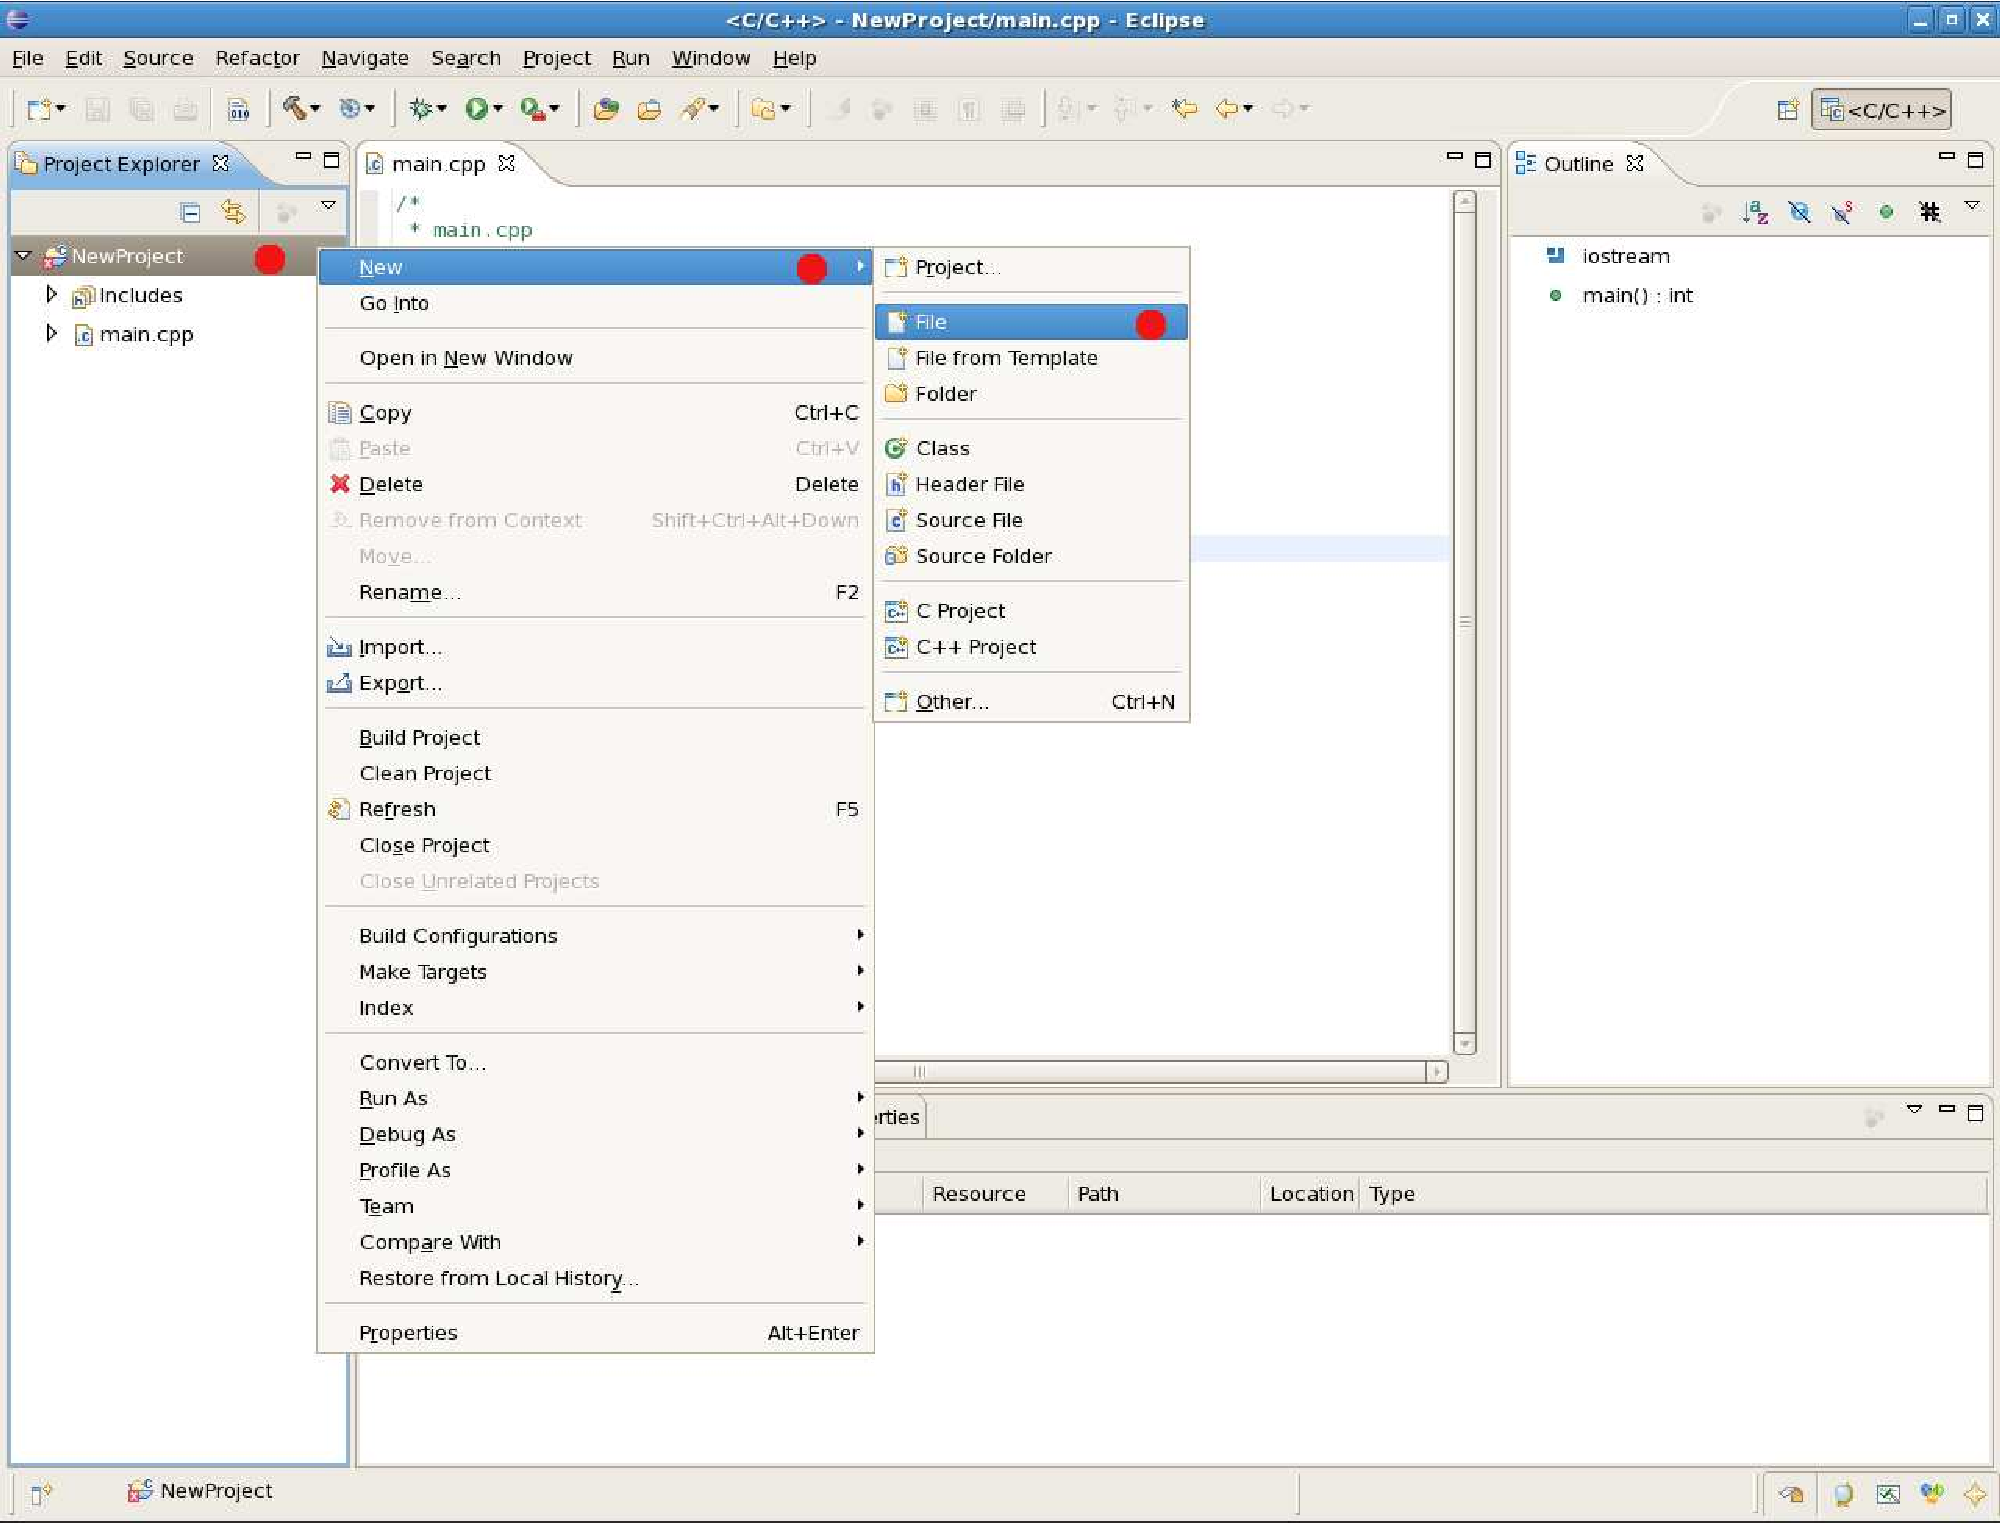
\includegraphics[width=0.95\textwidth]{./images/eclipse6}
    \end{figure}

\end{frame}

%---------------------------------------------------------------------------------

\begin{frame}[fragile]

    \frametitle{Eclipse: inserire il nome}

    \begin{figure}
        \centering
        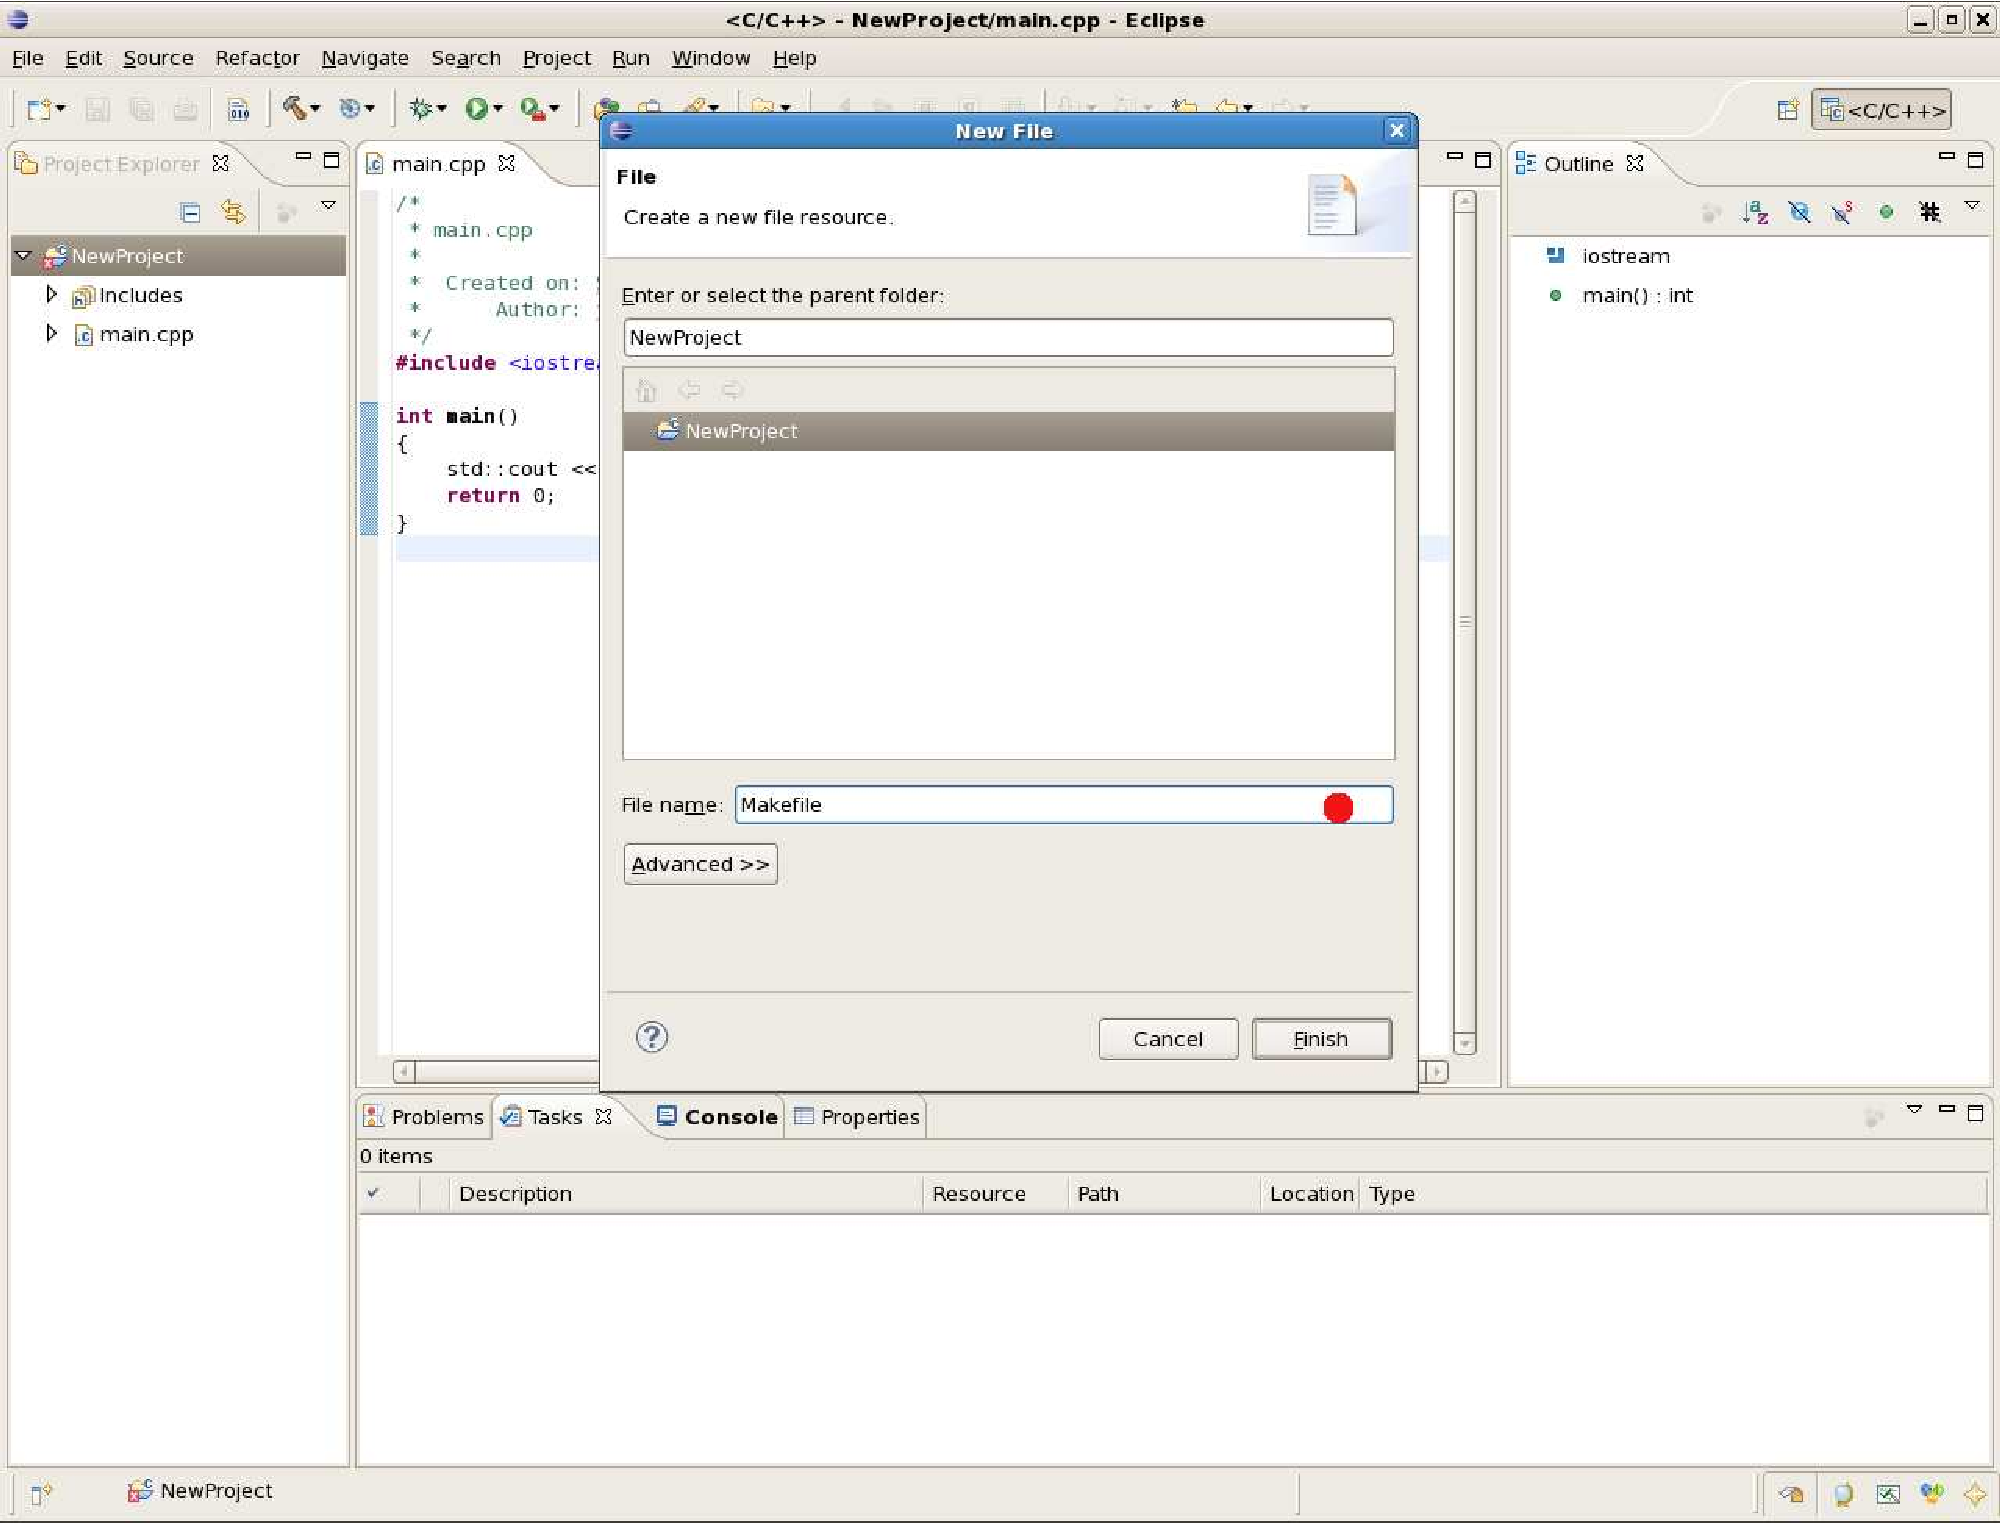
\includegraphics[width=0.95\textwidth]{./images/eclipse7}
    \end{figure}

\end{frame}

%---------------------------------------------------------------------------------

\begin{frame}[fragile]

    \frametitle{Eclipse: scrivere il Makefile}

    \begin{figure}
        \centering
        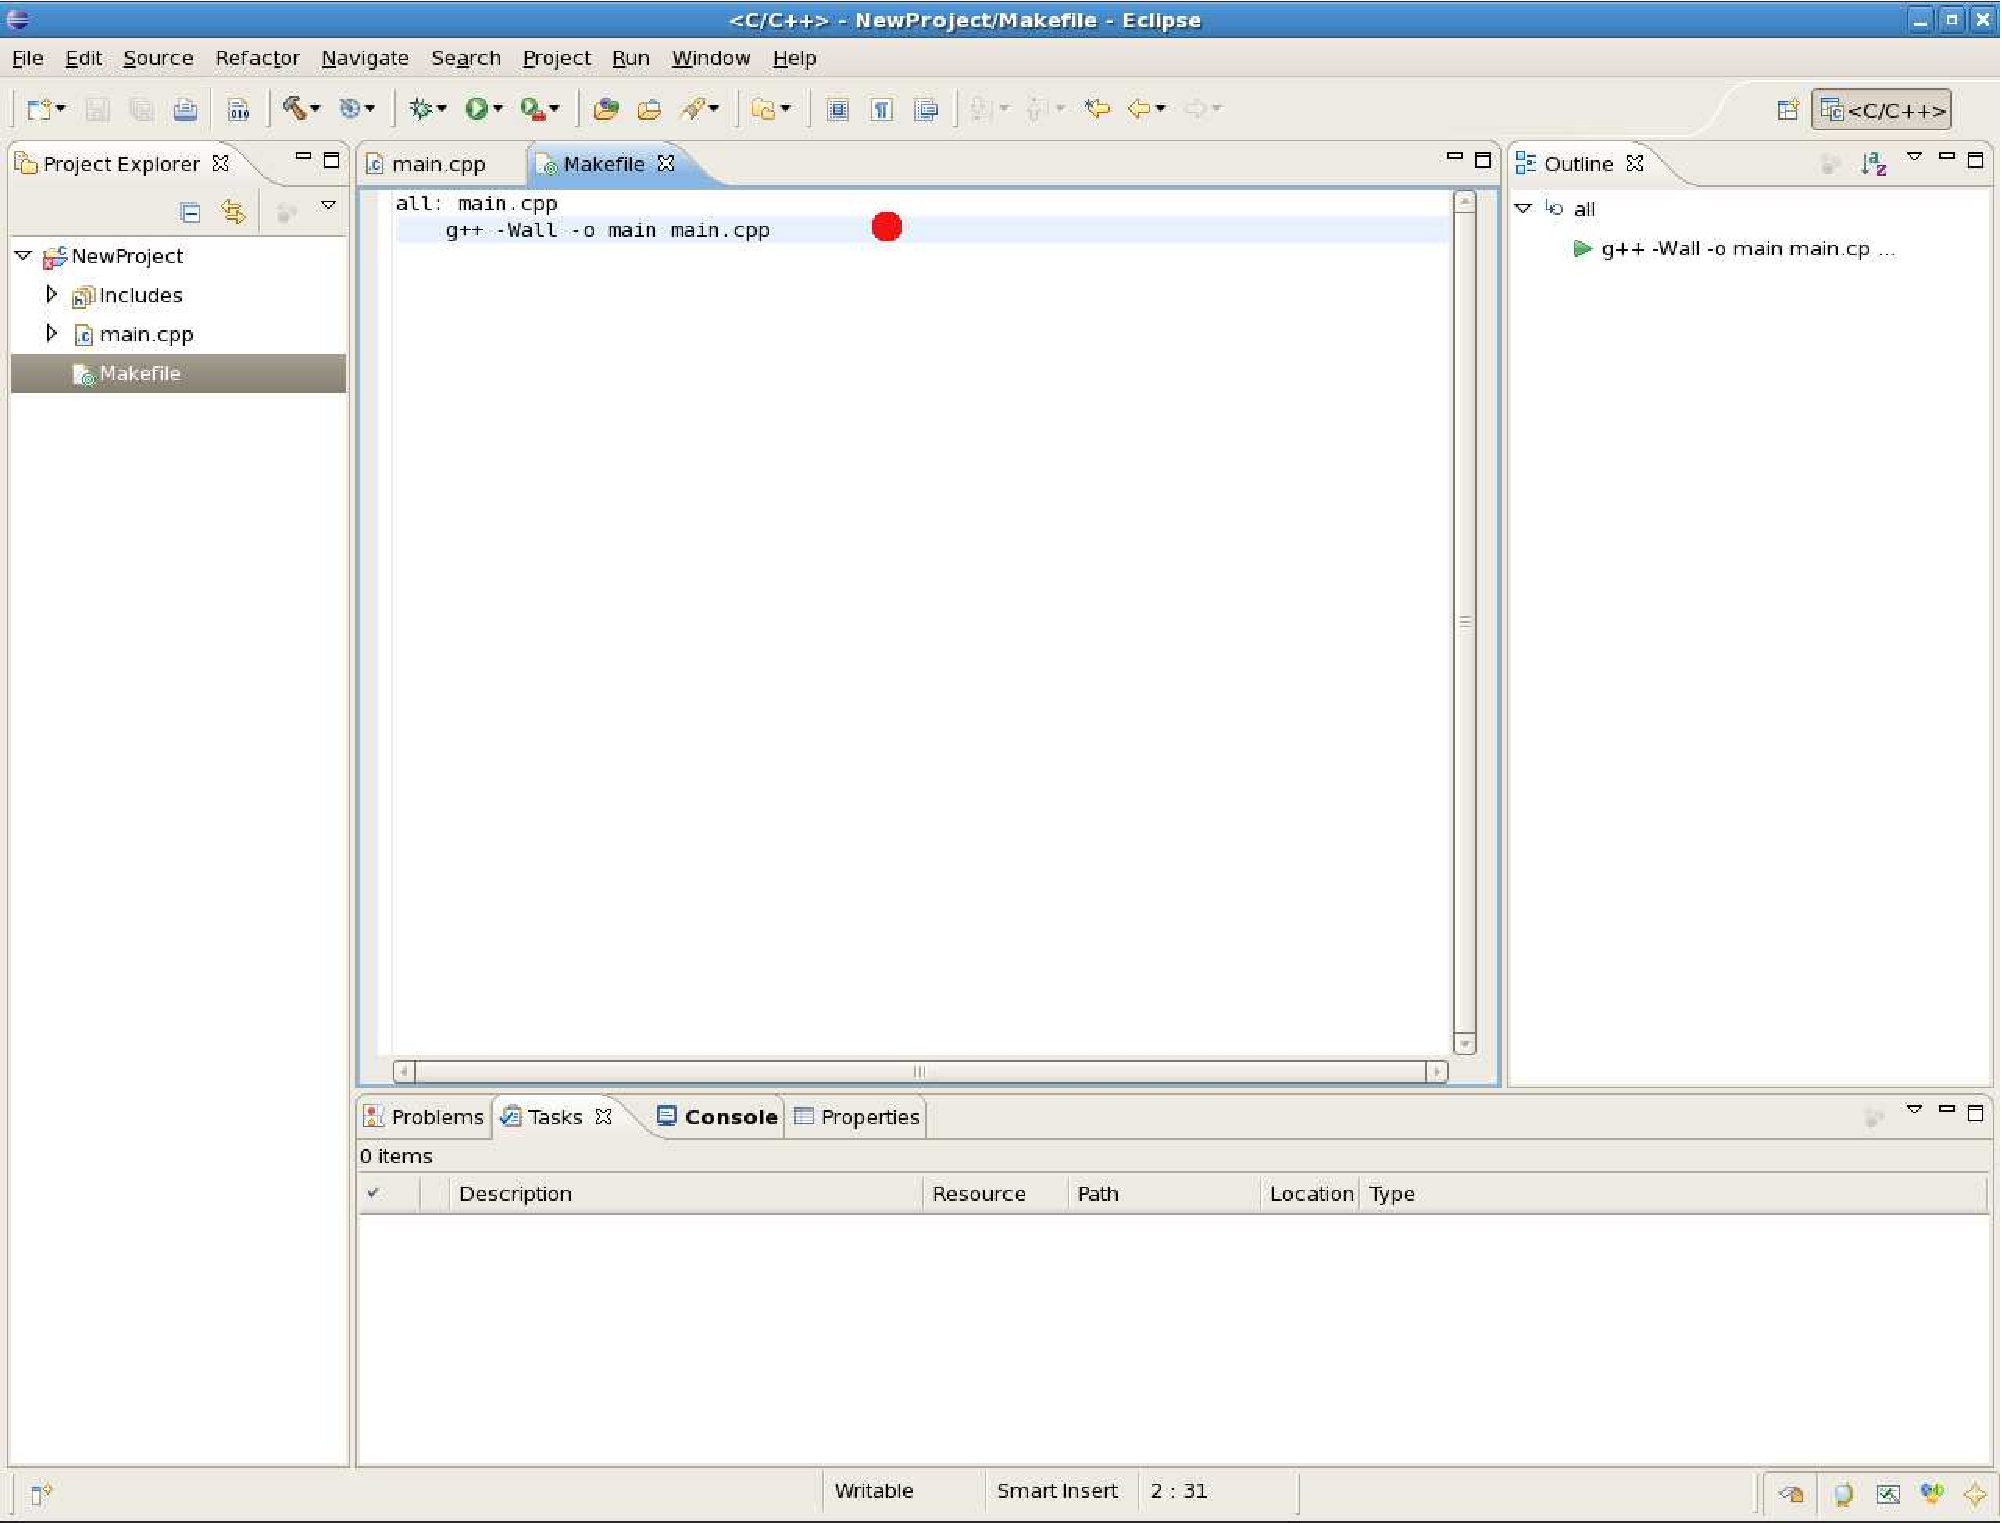
\includegraphics[width=0.95\textwidth]{./images/eclipse8}
    \end{figure}

\end{frame}

%---------------------------------------------------------------------------------

\begin{frame}[fragile]

    \frametitle{Eclipse: impostare la compilazione}

    \begin{figure}
        \centering
        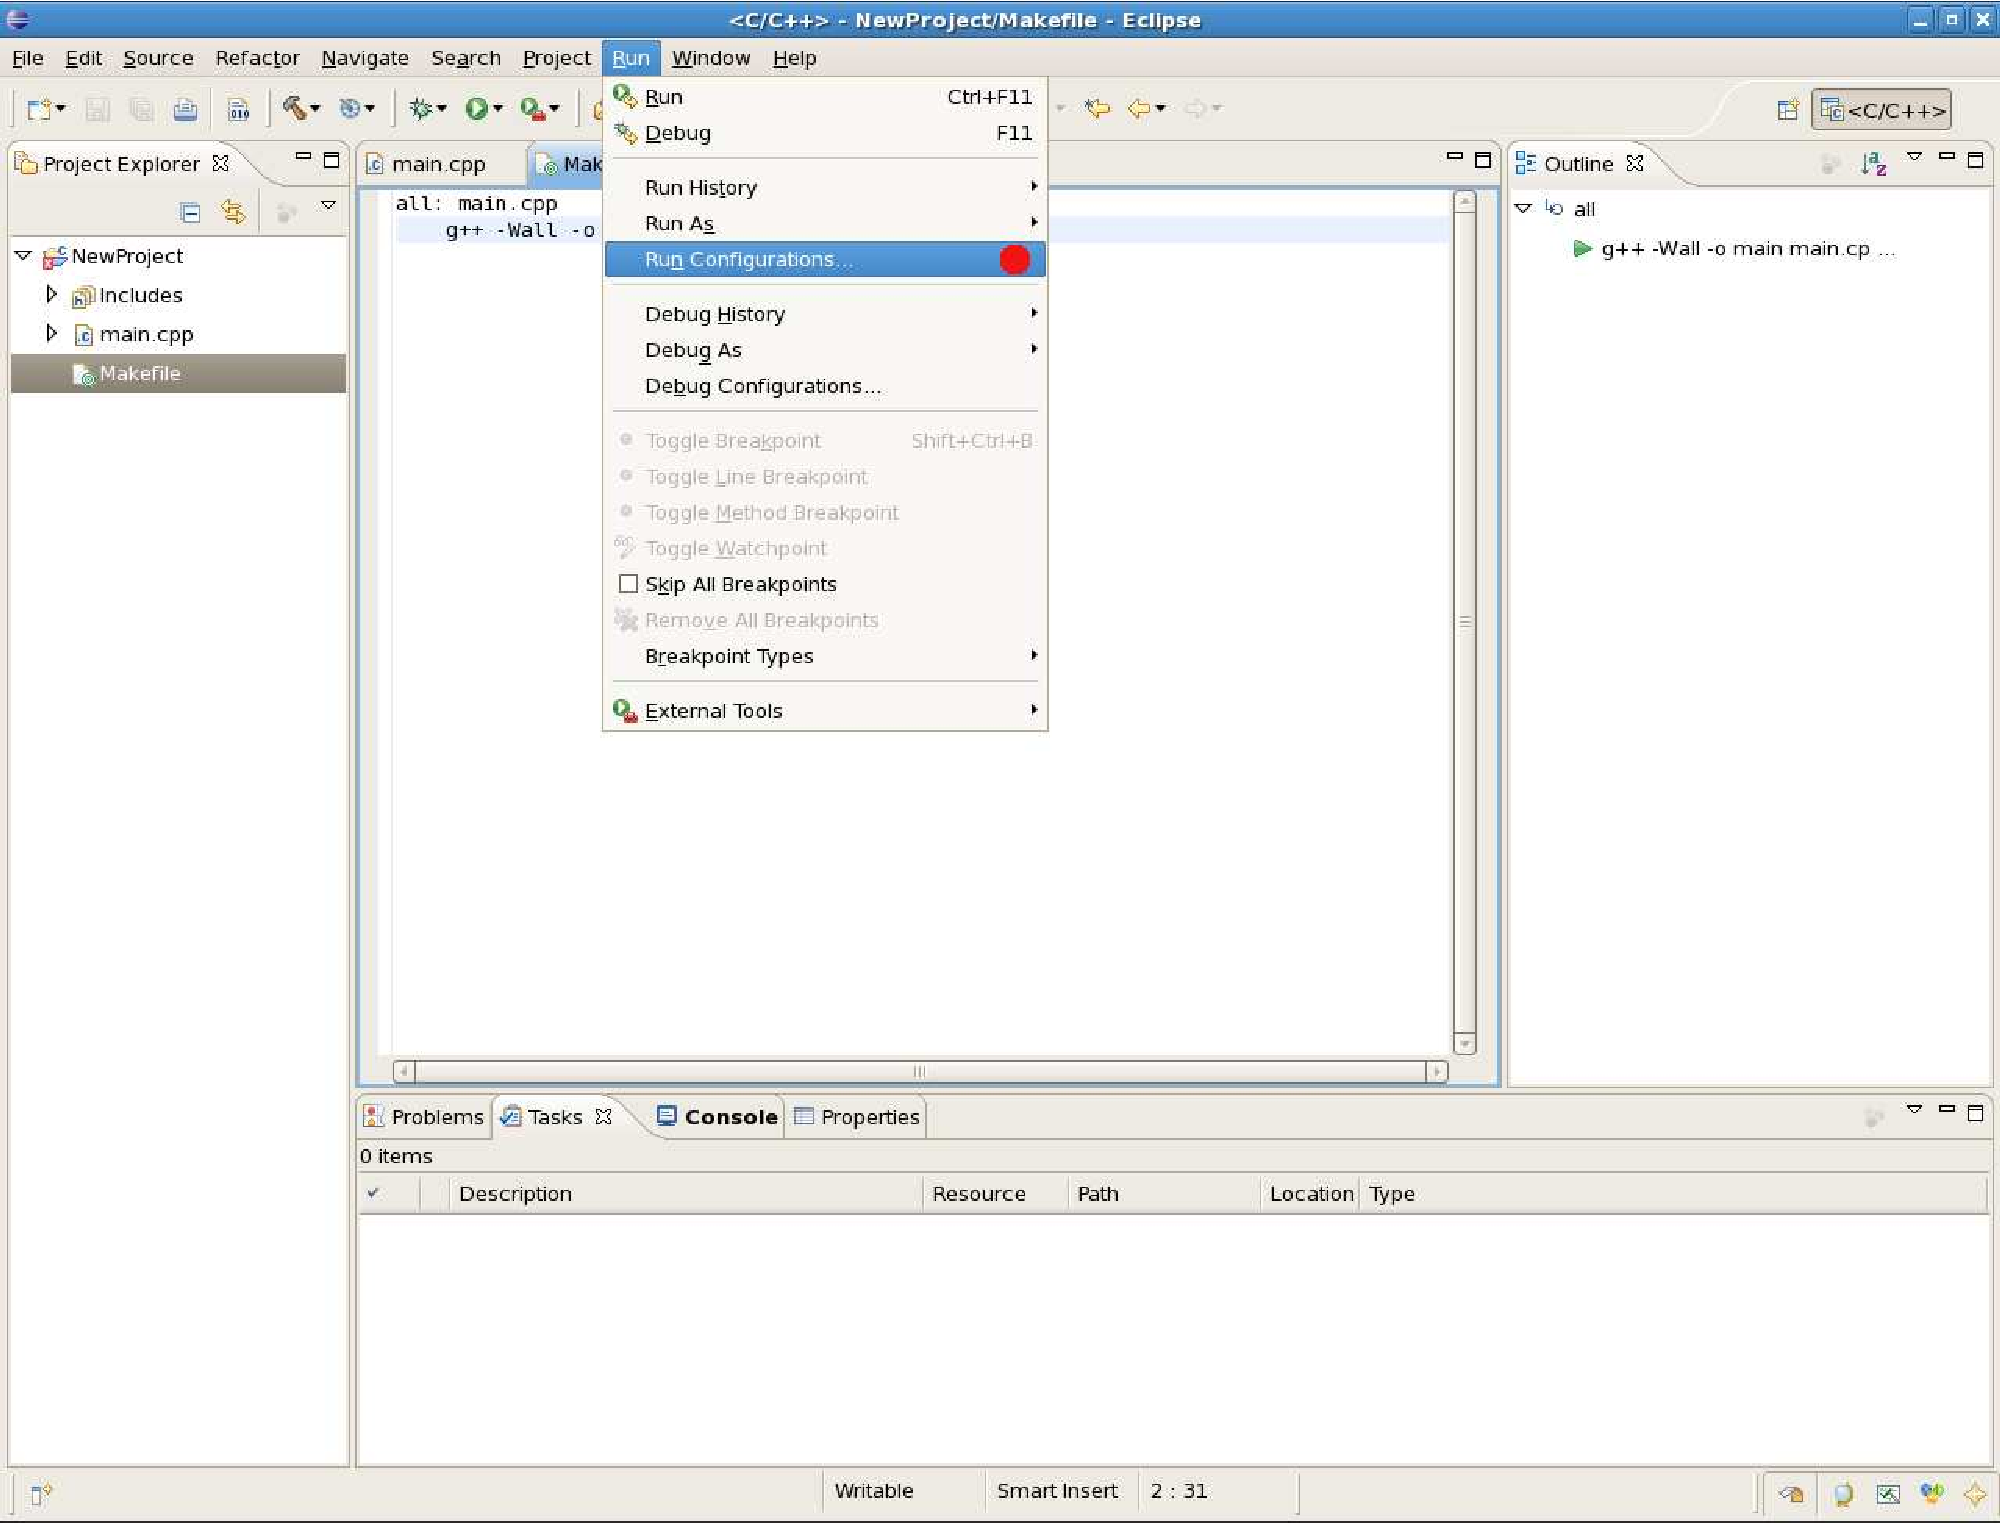
\includegraphics[width=0.95\textwidth]{./images/eclipse9}
    \end{figure}

\end{frame}

%---------------------------------------------------------------------------------

\begin{frame}[fragile]

    \frametitle{Eclipse: inserire il nome dell'eseguibile}

    \begin{figure}
        \centering
        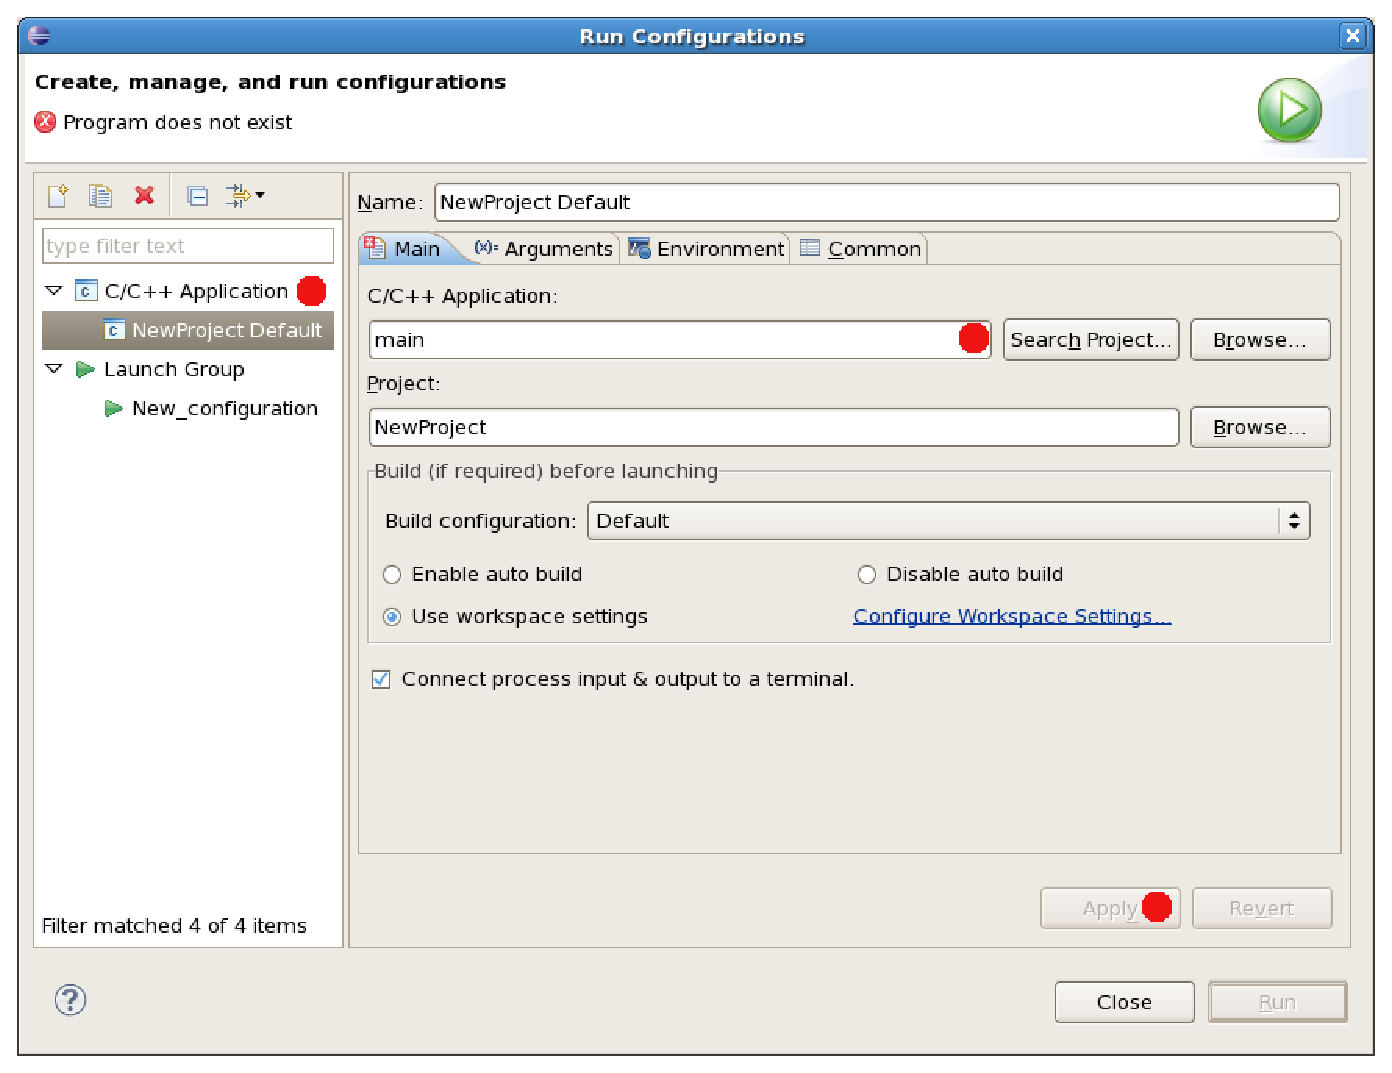
\includegraphics[width=0.95\textwidth]{./images/eclipse10}
    \end{figure}

\end{frame}

%---------------------------------------------------------------------------------

\begin{frame}[fragile]

    \frametitle{Eclipse: compilare e eseguire il programma}

    \begin{figure}
        \centering
        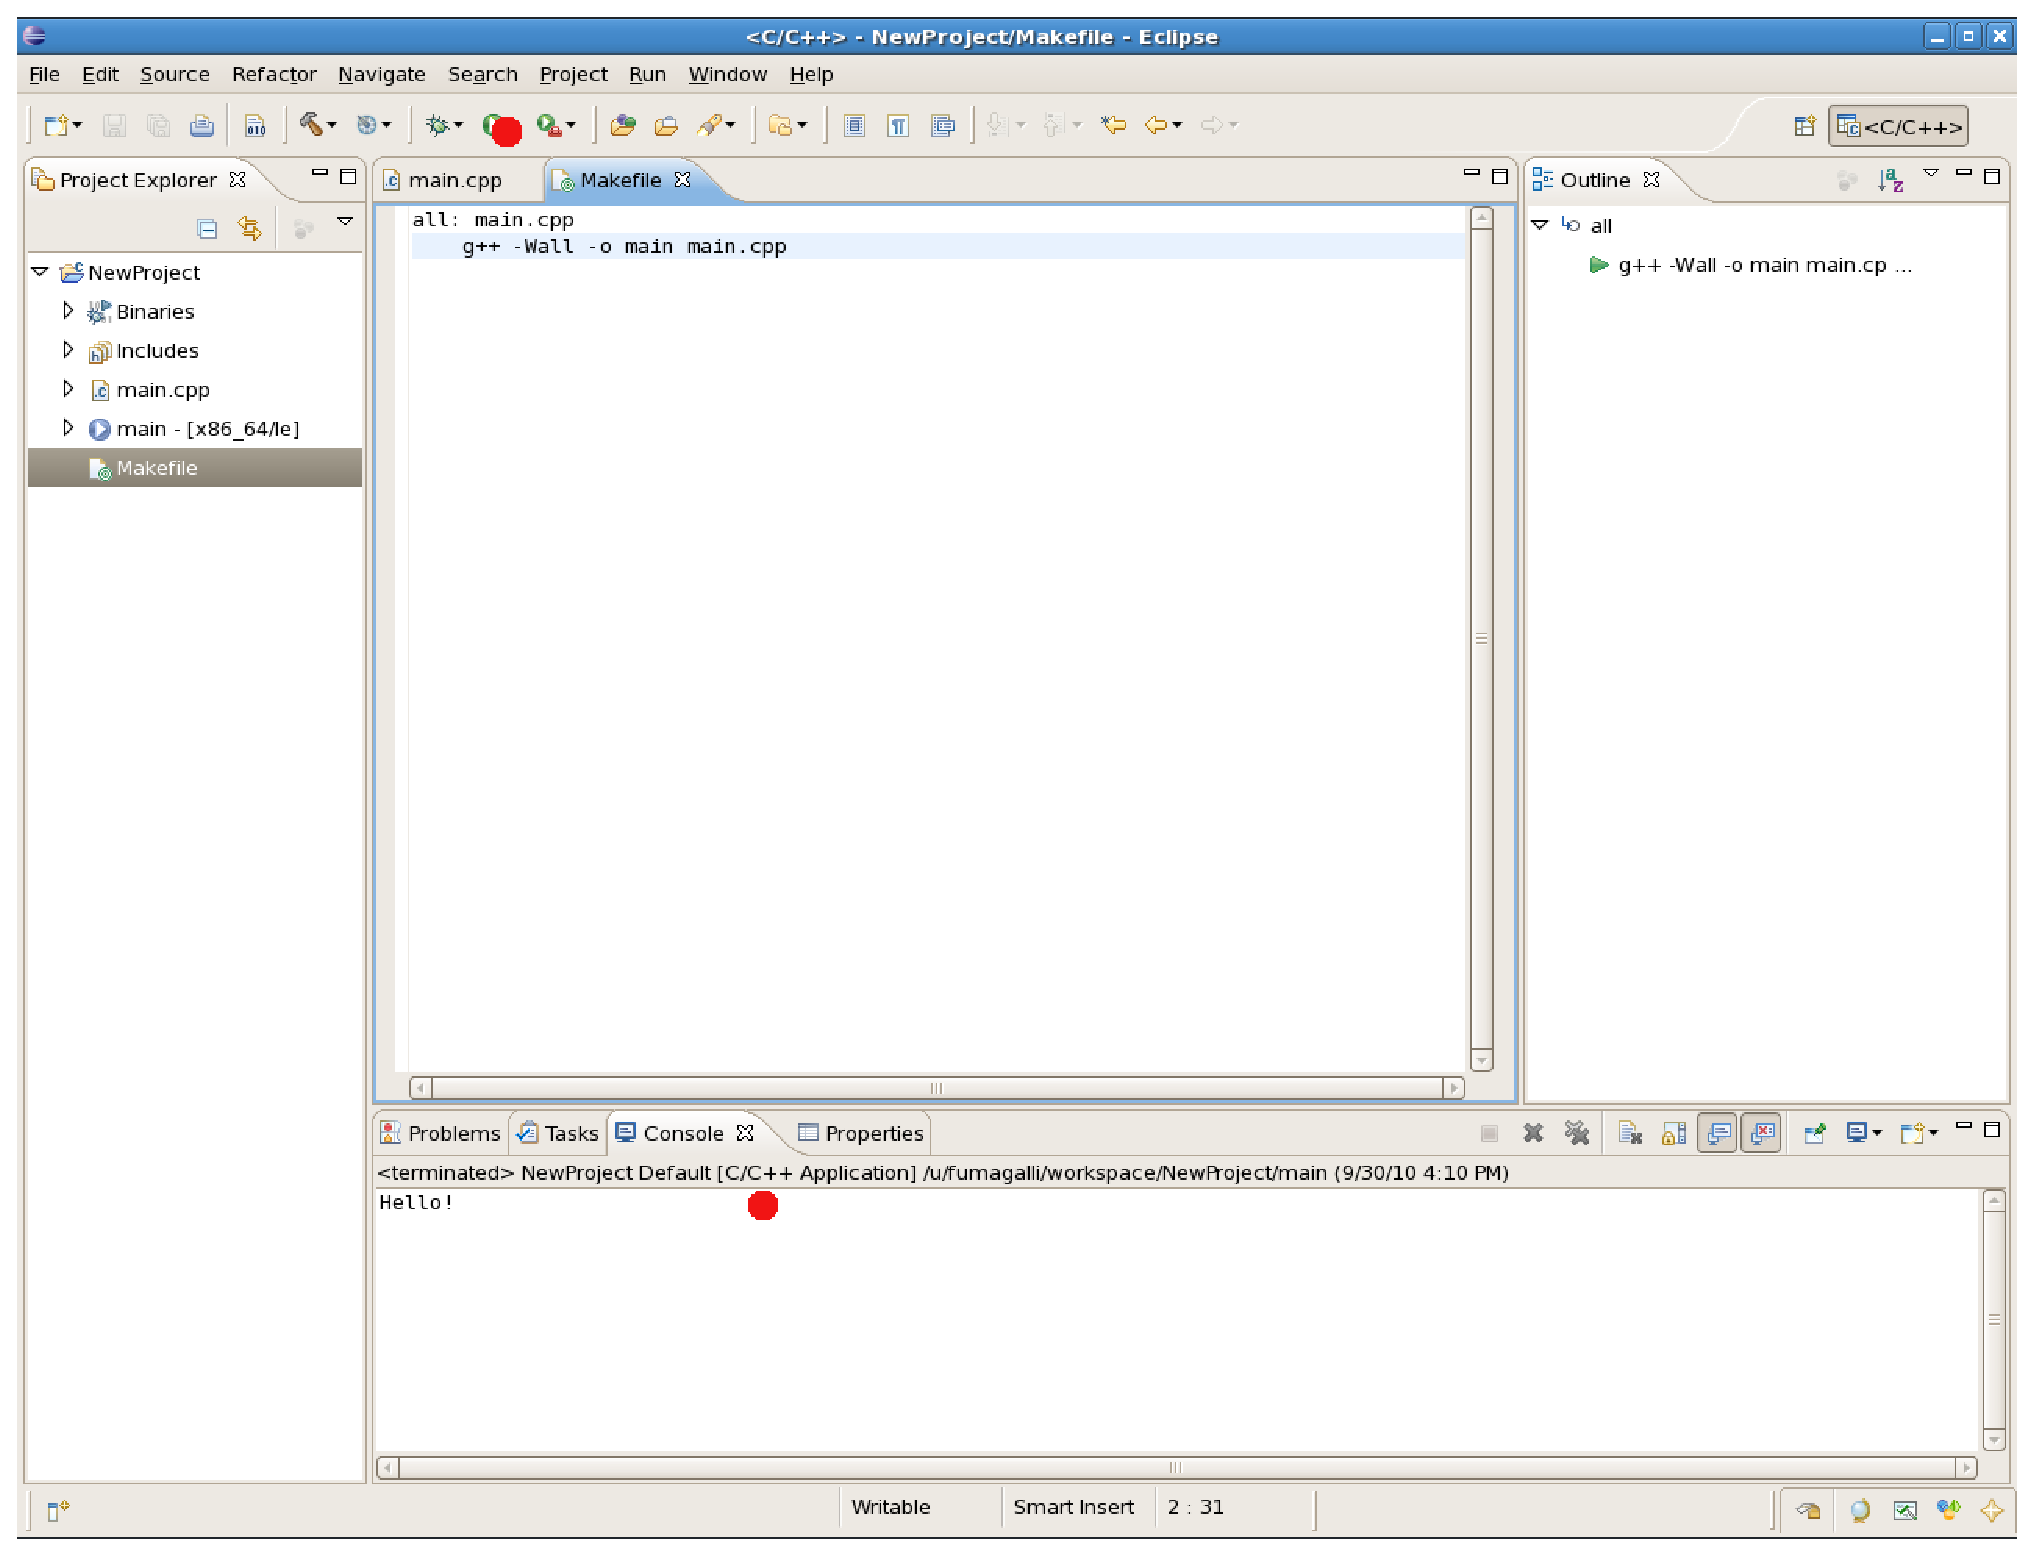
\includegraphics[width=0.95\textwidth]{./images/eclipse11}
    \end{figure}

\end{frame}

\end{document}
